\documentclass[11pt,tikz,border=5pt]{standalone}
\usepackage{amsmath}
\usepackage[compat=1.1.0]{tikz-feynman}
\usepackage[T1]{fontenc}
\usetikzlibrary{calc}
\tikzset{
  gluon/.style={draw=black,line width=.65pt,/tikzfeynman/gluon},
  wilson/.style={draw=black,line width=.45pt,double=white,double distance=1.7pt},
  cut/.style={draw=black,line width=.5pt,dash pattern=on 1.3pt off 1.7pt}}
\begin{document}
% Representative real interference cut. Wilson-line orientations and the
% conjugate contribution are specified separately in the operator definition.
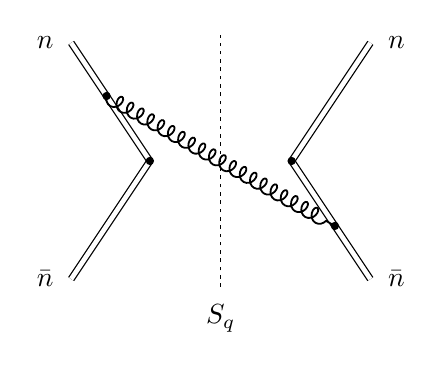
\begin{tikzpicture}
  \coordinate (O) at (.9,0);
  \coordinate (B) at (2.7,0);
  \coordinate (LN) at (-.1,1.5);
  \coordinate (LB) at (-.1,-1.5);
  \coordinate (RN) at (3.7,1.5);
  \coordinate (RB) at (3.7,-1.5);
  \coordinate (E) at ($(O)!.55!(LN)$);
  \coordinate (F) at ($(B)!.55!(RB)$);
  \draw[cut] (1.8,-1.6)--(1.8,1.6);
  \draw[wilson] (O)--(LN);
  \draw[wilson] (LB)--(O);
  \draw[wilson] (RN)--(B);
  \draw[wilson] (B)--(RB);
  \draw[gluon] (E)--(F);
  \foreach \point in {O,B,E,F}{\fill (\point) circle (1.5pt);}
  \node[anchor=east] at (-.2,1.5) {$n$};
  \node[anchor=east] at (-.2,-1.5) {$\bar n$};
  \node[anchor=west] at (3.8,1.5) {$n$};
  \node[anchor=west] at (3.8,-1.5) {$\bar n$};
  \node at (1.8,-2.0) {$S_q$};
\end{tikzpicture}
\end{document}
